\subsection*{Ноутбук + зарядка}
\addcontentsline{toc}{subsection}{Ноутбук + зарядка}

\textbf{Задание:}\\
Реализовать модель работы ноутбука при условии, что присутствует возможность зарядки.\\

\textbf{Решение:}\\
Для начала стоит с помощью элементов презентации нарисовать мышку и сам ноутбук. (Рисунок \ref{fig:notebook1})
\begin{figure}[h]
	\centering 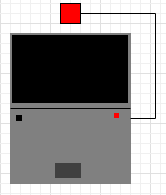
\includegraphics[scale=0.5]{notebook1}
	\caption{Визуализация ноутбука и мышки}
	\label{fig:notebook1}
\end{figure}

Далее была описана логика работы и построены диаграммы состояний. (Рисунок \ref{fig:notebook2})
\begin{figure}[h]
	\centering 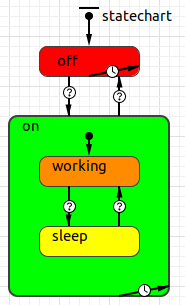
\includegraphics[scale=0.5]{notebook2}
	\caption{Диаграммы состояний}
	\label{fig:notebook2}
\end{figure}

Всего существуют два глобальных состояний: ноутбук включен и ноутбук выключен. Пока ноутбук включен, то у него постепенно расходуется заряд, если заряд ноутбука заканчивается, то он переходит в состояние выключения. Для отслеживания текущего состояния переменных у двух состояний есть внутренние переходы по таймауту, которые обновляются каждую секунду. Как только ноутбук подключается к зарядке, то им снова можно пользоваться.\\

Также в глобальном состоянии, когда ноутбук включен есть два внутренних: работает и в состоянии сна. Если не нажимать на кнопки на клавиатуре или на тачпад, то ноутбук перейдёт в состояния сна и продолжит потреблять зарядку.\\

Ещё у ноутбука есть кнопка включения и выключения, чтобы пользователь мог сам переключаться между состояниями.\\

Реализация логики одного из внутренних переходов ноутбука представлена ниже. (Рисунок \ref{fig:notebook3})
\begin{figure}[h]
	\centering 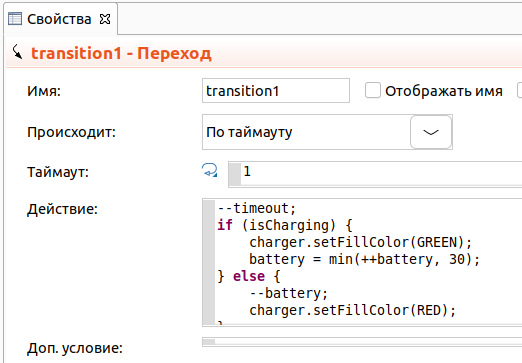
\includegraphics[scale=0.5]{notebook3}
	\caption{Реализация логики внутреннего перехода в ноутбуке}
	\label{fig:notebook3}
\end{figure}

Таким образом, была реализована модель, имитирующая работу ноутбука с зарядкой.\\